\subsection{Greedy Best-First Search}
\noindent Greedy Best-First Search is similar to A* algorithm. The difference is that the vertices in the priority queue are ordered only by the estimated remaining distance to the solution. It has to be noted that complete best first search is not optimal.

\begin{figure}
	\centering
	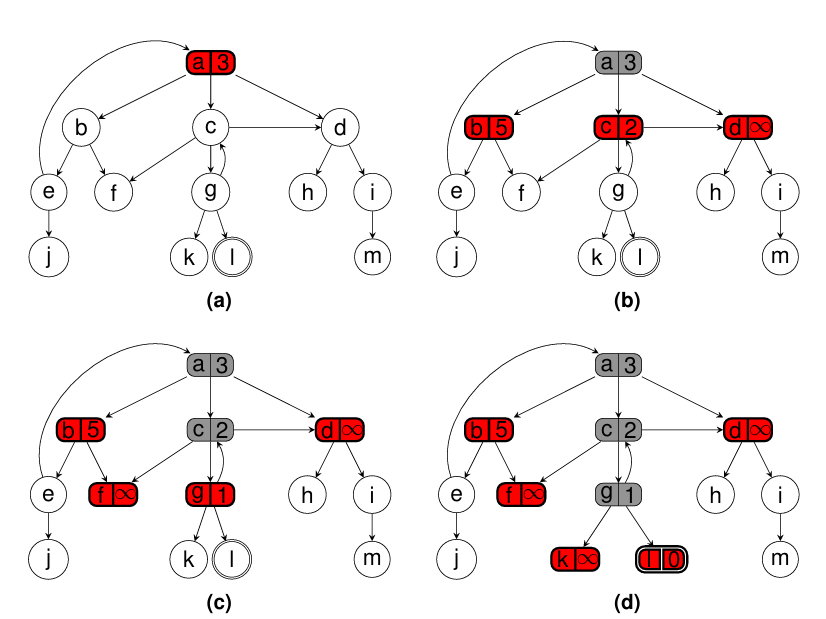
\includegraphics[width=0.8\textwidth]{./imgs/gbfs.png}
	\caption{Greedy Best-First Search}
	\label{fig:GBFS}
\end{figure}

\subsubsection{Pseudocode}
\begin{algorithm}[H]
	\caption{Greedy Best-First Search (\textit{start, goal, heuristic})}
	\label{alg:gbfs}
	\begin{algorithmic}[1]
	\State priority queue $\gets$ [(start, heuristic(start))]
	\While {priority queue is not empty}
		\State node $\gets$ dequeue(priority queue)
		\If {node = goal}
			\State return path
		\EndIf
		\ForAll {neighbor in valid moves}
			\If {neighbor not visited}
				\State mark neighbor as visited
				\State enqueue(priority queue, (neighbor, heuristic(neighbor)))
			\EndIf
		\EndFor
	\EndWhile
	\State return failure
	\end{algorithmic}
\end{algorithm}

\subsubsection{Time and Space Complexity}
